\documentclass[12pt]{article}
\usepackage[margin=1in]{geometry}
\usepackage{amsfonts,amsmath,amssymb}
\usepackage{multicol}
\usepackage{graphicx}
\usepackage{float}
\usepackage[nottoc, notlot, notlof]{tocbibind}
\usepackage{hyperref}
\usepackage{enumitem}
\usepackage{caption}
\usepackage{subcaption}
\usepackage[T1]{fontenc}
\usepackage{rotating}

\begin{document}
	\begin{center}
		\Large{\textbf{Magnetic Mirror Effect in Magnetron Plasma:}} \\
		\Large{\textbf{Modeling of Plasma Parameters}}
	\end{center}
	\noindent \Large{\textbf{Controlling Plasma stream with Helmholtz coils}} \normalsize \vspace{0.2cm}\\
	\noindent We now perform two studies with our setup.\\
	\noindent\textbf{Simulation data}
	\begin{itemize}
		\item 100 particles of Hydrogen ions (relative atomic mass: 1.008 g mol$^{-1}$).
		\item Duration of 1 step of update: 0.001 ms
		\item Number of steps: 3 x 100 = 300
		\item Total duration of simulation = 0.3 ms
	\end{itemize}
	\section{Study 2: Familiar distributions}
	For this study we use the following data: \\
	\noindent \textbf{Sampling of the Initial Positions and Velocities of the particles}
	\begin{itemize}
		\item Speeds are sampled from a Maxwellian distribution with plasma temperature 10000 K.
		\item Velocity directions are sampled from uniform distribution.
		\item Positions are sampled such that all particles start at [-0.5, 0, 0] (A box 1m x 1m x 1m from [-0.5, -0.5, -0.5] to	[0.5, 0.5, 0.5] maybe considered for reference)
	\end{itemize}
	\noindent We use the standard Maxwellian distribution for the initial speeds of the particles and have all particles start at the same position.
	\subsection{Magnetic field along a fixed axis, with constant current}
	For the first part of this study, we use the following field configurations.\\
	\noindent \textbf{Configurations of the Electric and Magnetic Fields}
	\begin{itemize}
		\item Magnetic field due to a Helmholtz coil (number of turns: 1000 in each coil, radius: 0.1 m): for 100  steps each \\ 
		first 20A current, orientation along
		the $z$-axis [0,0,1] \\
		second -20A current, orientation along
		the $z$-axis [0,0,1] \\
		third 20A current, orientation along
		the $z$-axis [0,0,1].
		\item Electric field constantly set to 0.
	\end{itemize}
	\noindent We see that we always use the coil oriented in the $z$-direction and we change the direction of the current while keeping the amplitude at a constant value of 20 A. We get the following results. First we plot the positions and components of positions of a particle in the simulation.
	\begin{figure}[H]
		\begin{multicols}{2}
			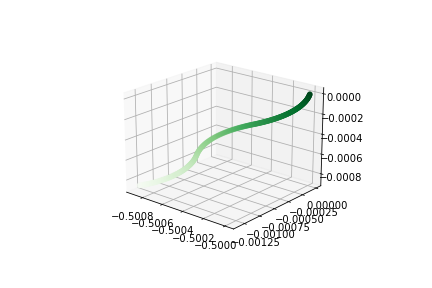
\includegraphics[width=\linewidth, height=6cm]{ps2Bz.png} \caption{position} \label{ps2Bz} \par
			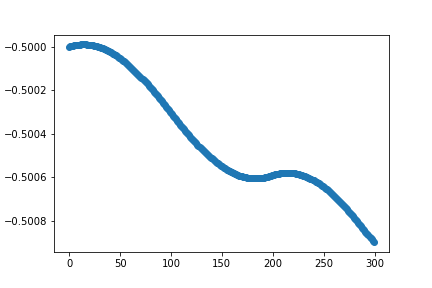
\includegraphics[width=\linewidth, height=6cm]{psx2Bz.png} \caption{$x$-component of position} \label{psx2Bz} \par
		\end{multicols}
	\end{figure}
	\begin{figure}[H]
		\begin{multicols}{2}
			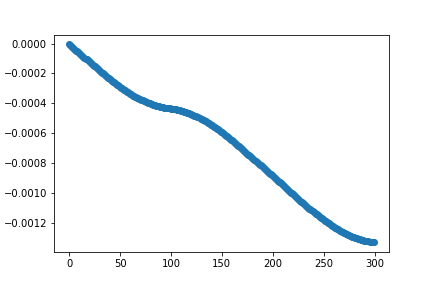
\includegraphics[width=\linewidth, height=6cm]{psy2Bz.png} \caption{$y$-component of position} \label{psy2Bz} \par
			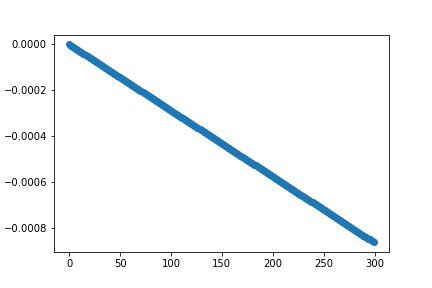
\includegraphics[width=\linewidth, height=6cm]{psz2Bz.png} \caption{$z$-component of position} \label{psz2Bz} \par
		\end{multicols}
	\end{figure}
	\noindent We see in figure (\ref{ps2Bz}), that the trajectory has three regions of curves which correspond to the three epochs of the positive, negative and then positive sign of the magnetic field. We see the same pattern of three curves in figures (\ref{psx2Bz}) and (\ref{psy2Bz}) and they appear to be out of phase with respect to one another. Things become more clear when we look at the velocities, as the change in the velocities caused by acceleration due to the fields (only the magnetic field is non zero in our case) is more intuitive. So now let's plot the velocities and components of velocities of the same particle.
	\begin{figure}[H]
		\begin{multicols}{2}
			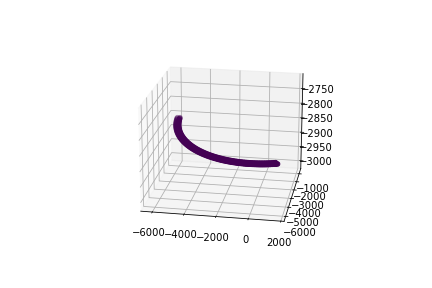
\includegraphics[width=\linewidth, height=6cm]{vs2Bz.png} \caption{velocity} \label{vs2Bz} \par
			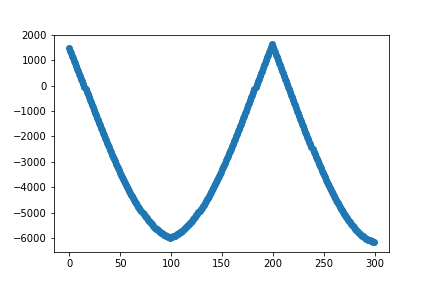
\includegraphics[width=\linewidth, height=6cm]{vsx2Bz.png} \caption{$x$-component of velocity} \label{vsx2Bz} \par
		\end{multicols}
	\end{figure}
	\begin{figure}[H]
		\begin{multicols}{2}
			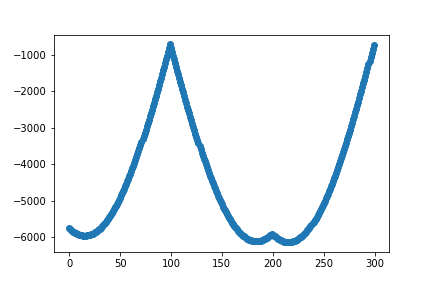
\includegraphics[width=\linewidth, height=6cm]{vsy2Bz.png} \caption{$y$-component of velocity} \label{vsy2Bz} \par
			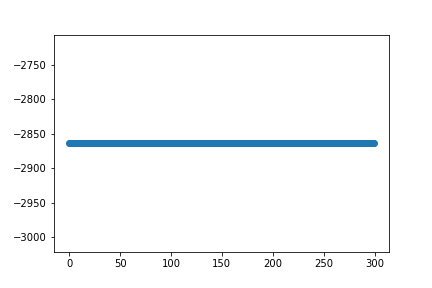
\includegraphics[width=\linewidth, height=6cm]{vsz2Bz.png} \caption{$z$-component of velocity} \label{vsz2Bz} \par
		\end{multicols}
	\end{figure}
	\noindent We see in figure (\ref{vsz2Bz}) that the $z$-component of the velocity remains constant, as the acceleration along the $z$-axis is zero since the magnetic field is along the $z$-axis and the $\mathbf{B} \times \boldsymbol{v}$ acceleration caused by the magnetic field is perpendicular to the direction of the magnetic field. The acceleration is nonzero only in the $x$-$y$ plane. In figures (\ref{vsx2Bz}) and (\ref{vsy2Bz}) we see two events of non-smooth change in the velocity components at $100^{th}$ and $200^{th}$ update steps which correspond to the change in the sign of the current supplied to the coil, hence the direction of the magnetic field and therefore the direction of the acceleration. Otherwise we see the harmonic oscillation velocity profile in each epoch, which would describe such a situation. We now plot the positions and the components of positions for 10 particles in the simulation.
	\begin{figure}[H]
		\begin{multicols}{2}
			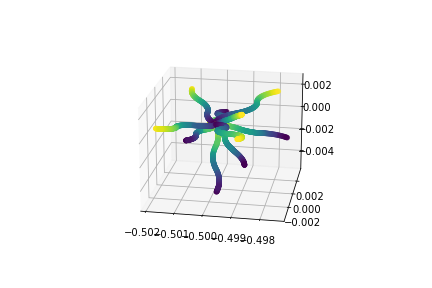
\includegraphics[width=\linewidth, height=6cm]{multips2Bz.png} \caption{positions} \label{multips2Bz} \par
			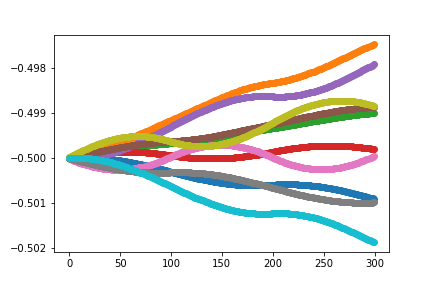
\includegraphics[width=\linewidth, height=6cm]{multipsx2Bz.png} \caption{$x$-component of positions} \label{multipsx2Bz} \par
		\end{multicols}
	\end{figure}
	\begin{figure}[H]
		\begin{multicols}{2}
			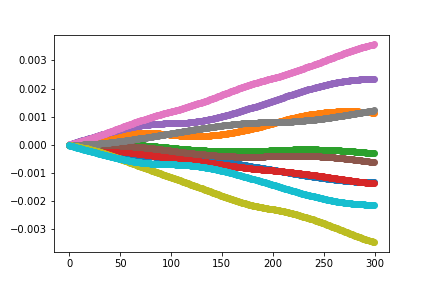
\includegraphics[width=\linewidth, height=6cm]{multipsy2Bz.png} \caption{$y$-component of positions} \label{multipsy2Bz} \par
			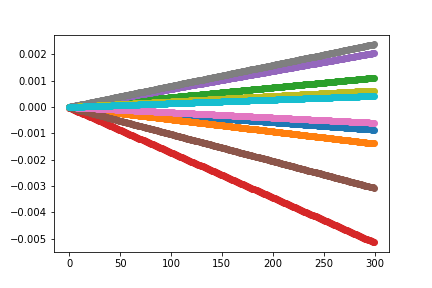
\includegraphics[width=\linewidth, height=6cm]{multipsz2Bz.png} \caption{$z$-component of positions} \label{multipsz2Bz} \par
		\end{multicols}
	\end{figure}
	\noindent Like with the single particle, we see the trajectories curve three times in figure (\ref{multips2Bz}), and figures (\ref{multipsx2Bz}) and (\ref{multipsy2Bz}). We also plot the velocities and the components of velocities for the same 10 particles.
	\begin{figure}[H]
		\begin{multicols}{2}
			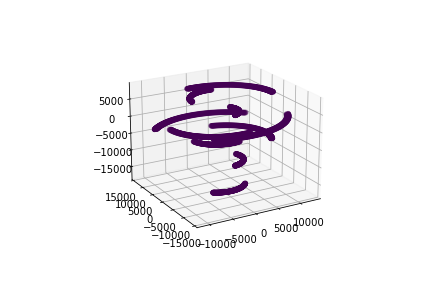
\includegraphics[width=\linewidth, height=6cm]{multivs2Bz.png} \caption{velocities} \label{multivs2Bz} \par
			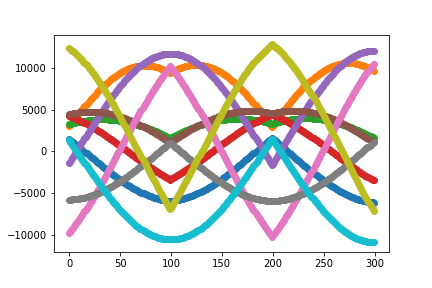
\includegraphics[width=\linewidth, height=6cm]{multivsx2Bz.png} \caption{$x$-component of velocities} \label{multivsx2Bz} \par
		\end{multicols}
	\end{figure}
	\begin{figure}[H]
		\begin{multicols}{2}
			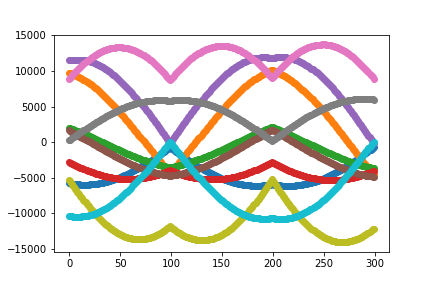
\includegraphics[width=\linewidth, height=6cm]{multivsy2Bz.png} \caption{$y$-component of velocities} \label{multivsy2Bz} \par
			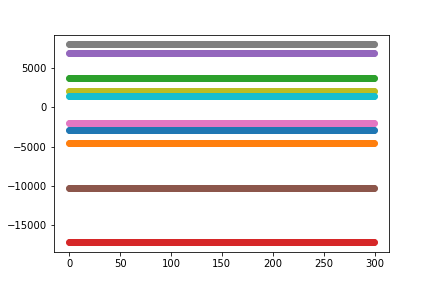
\includegraphics[width=\linewidth, height=6cm]{multivsz2Bz.png} \caption{$z$-component of velocities} \label{multivsz2Bz} \par
		\end{multicols}
	\end{figure}
	\noindent Like with the single particle we see in figure (\ref{multivsz2Bz}) that the $z$-components of the velocities remain constant and in figures (\ref{multivsx2Bz})  and (\ref{multivsy2Bz}) that the $x$ and $y$ components of the velocities change non-smoothly in the $100^{th}$ and the $200^{th}$ iterations while they follow harmonic oscillations in each epoch of unchanging magnetic fields. 

	\subsection{Magnetic field with changing current and orientation}
	For the second part of the study, we use a slightly different magnetic field configuration. We change the axis of the coil and also the current. \\
	\noindent \textbf{Configurations of the Electric and Magnetic Fields}
	\begin{itemize}
		\item Magnetic field due to a Helmholtz coil (number of turns: 1000 in each coil, radius: 0.1 m): for 100  steps each \\ 
		first 100A current, orientation along
		the $z$-axis [0,0,1] \\
		second -20A current, orientation along the $x$-axis [1,0,0] \\
		third 50A current,
		orientation along the $y$-axis [0,1,0].
		\item Electric field constantly set to 0.
	\end{itemize}
	\noindent We first plot the positions and the components of positions for a particle in the simulation.
	\begin{figure}[H]
		\begin{multicols}{2}
			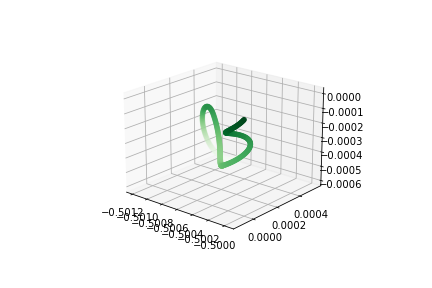
\includegraphics[width=\linewidth, height=6cm]{ps2.png} \caption{position} \label{ps2} \par
			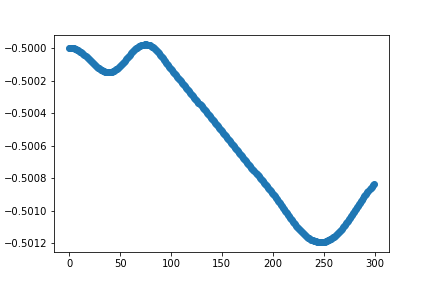
\includegraphics[width=\linewidth, height=6cm]{psx2.png} \caption{$x$-component of position} \label{psx2} \par
		\end{multicols}
	\end{figure}
	\begin{figure}[H]
		\begin{multicols}{2}
			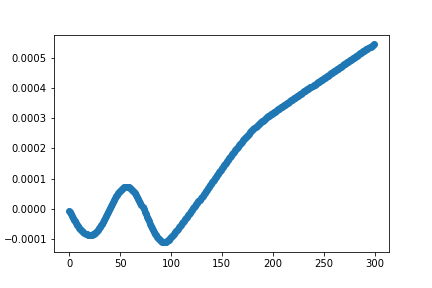
\includegraphics[width=\linewidth, height=6cm]{psy2.png} \caption{$y$-component of position} \label{psy2} \par
			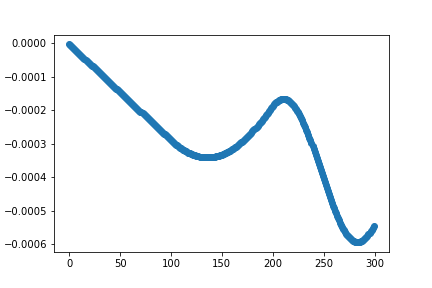
\includegraphics[width=\linewidth, height=6cm]{psz2.png} \caption{$z$-component of position} \label{psz2} \par
		\end{multicols}
	\end{figure}
	\noindent Because we change the direction of the magnetic field from along the $z$-axis to along the $x$-axis and then along the $y$-axis, in figures ($\ref{psx2}$), (\ref{psy2}) and (\ref{psz2}), we see two epoch of curves and one epoch of straight line. In figure (\ref{ps2}) we see one loop about the $y$ quite clearly while the other two curves are less clear to understand. Let's plot the velocities and the components of velocities for the same particle to see if we can understand better.
	\begin{figure}[H]
		\begin{multicols}{2}
			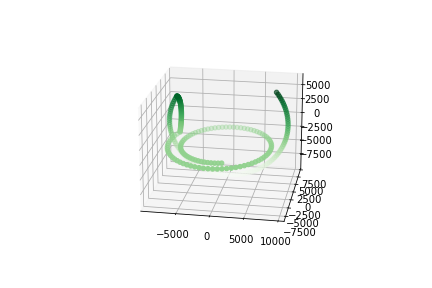
\includegraphics[width=\linewidth, height=6cm]{vs2.png} \caption{velocity} \label{vs2} \par
			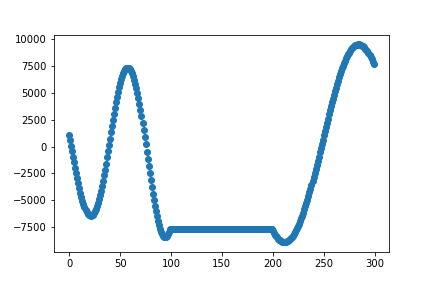
\includegraphics[width=\linewidth, height=6cm]{vsx2.png} \caption{$x$-component of velocity} \label{vsx2} \par
		\end{multicols}
	\end{figure}
	\begin{figure}[H]
		\begin{multicols}{2}
			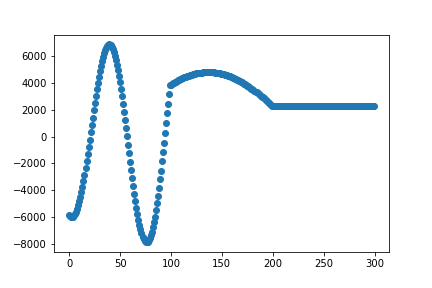
\includegraphics[width=\linewidth, height=6cm]{vsy2.png} \caption{$y$-component of velocity} \label{vsy2} \par
			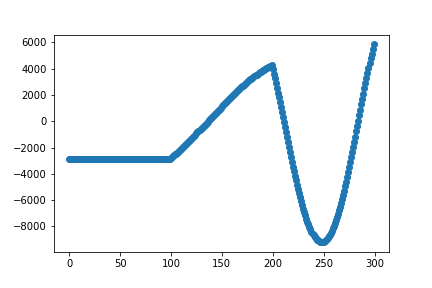
\includegraphics[width=\linewidth, height=6cm]{vsz2.png} \caption{$z$-component of velocity} \label{vsz2} \par
		\end{multicols}
	\end{figure}
	\noindent We see two epochs of curved lines and one epoch of constant components of velocity in figures (\ref{vsx2}), (\ref{vsy2}) and (\ref{vsz2}). The corresponding component of the velocity stays constant when the direction of the magnetic field is along that axis, otherwise the sharpness of the curves depends on the current applied in the coil. In figure (\ref{vs2}) we can see three loops about the three axes, which correspond to harmonic motion in the plane perpendicular to the magnetic field in each epoch. We now plot the positions and the components of positions for 10 particles in the simulation.
	\begin{figure}[H]
		\begin{multicols}{2}
			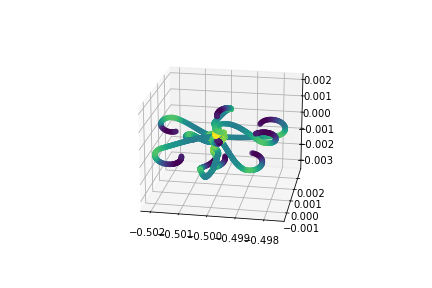
\includegraphics[width=\linewidth, height=6cm]{multips2.png} \caption{positions} \label{multips2} \par
			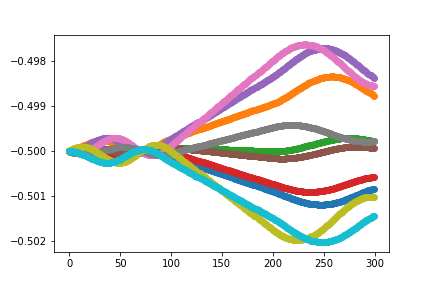
\includegraphics[width=\linewidth, height=6cm]{multipsx2.png} \caption{$x$-component of positions} \label{multipsx2} \par
		\end{multicols}
	\end{figure}
	\begin{figure}[H]
		\begin{multicols}{2}
			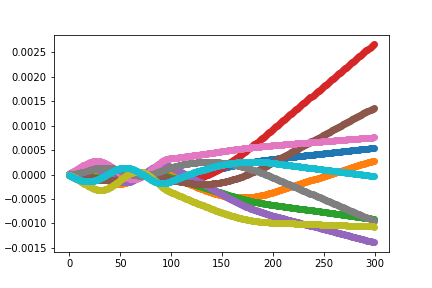
\includegraphics[width=\linewidth, height=6cm]{multipsy2.png} \caption{$y$-component of positions} \label{multipsy2} \par
			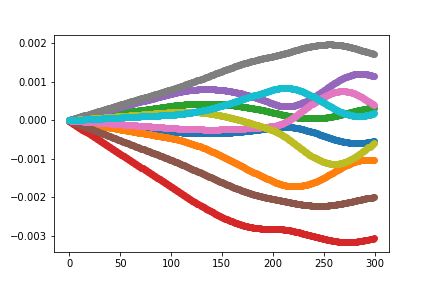
\includegraphics[width=\linewidth, height=6cm]{multipsz2.png} \caption{$z$-component of positions} \label{multipsz2} \par
		\end{multicols}
	\end{figure}
	\noindent Like with the single particle, we see two epochs of curves and one epoch of straight line in figures (\ref{multipsx2}), (\ref{multipsy2}) and (\ref{multipsz2}), and in figure (\ref{multips2}) we see one of the arcs (in what looks like the arms of and octopus) quite clearly for some of the particles. We also plot the velocities and the components of velocities for the same 10 particles.
	\begin{figure}[H]
		\begin{multicols}{2}
			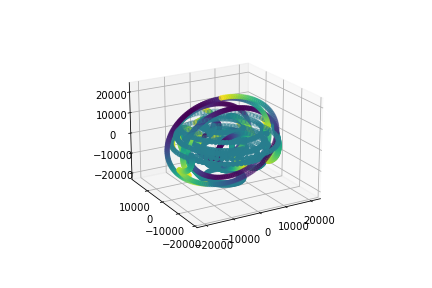
\includegraphics[width=\linewidth, height=6cm]{multivs2.png} \caption{velocities} \label{multivs2} \par
			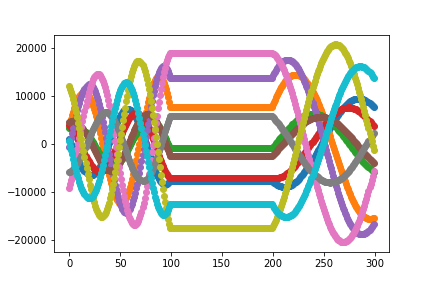
\includegraphics[width=\linewidth, height=6cm]{multivsx2.png} \caption{$x$-component of velocities} \label{multivsx2} \par
		\end{multicols}
	\end{figure}
	\begin{figure}[H]
		\begin{multicols}{2}
			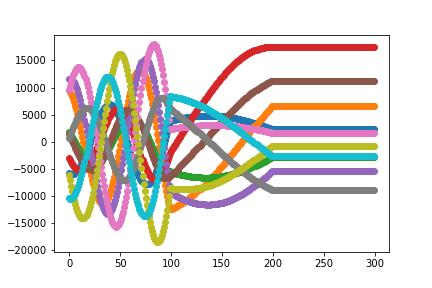
\includegraphics[width=\linewidth, height=6cm]{multivsy2.png} \caption{$y$-component of velocities} \label{multivsy2} \par
			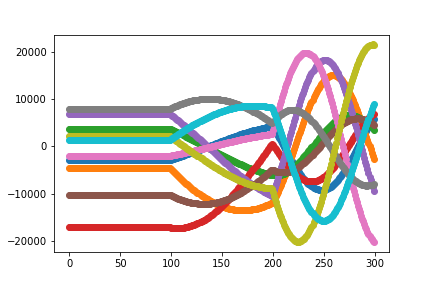
\includegraphics[width=\linewidth, height=6cm]{multivsz2.png} \caption{$z$-component of velocities} \label{multivsz2} \par
		\end{multicols}
	\end{figure}
	\noindent Although figure (\ref{multivs2}) is quite messy, we can notice loop-like circular trajectories. In figures (\ref{multivsx2}), (\ref{multivsy2}) and (\ref{multivsz2}) we see two epochs of harmonic motion and one epoch of constant component of velocity when the magnetic field is along the corresponding axis, like with the single particle plots.
	
	\section{Study 3: Different distributions}
	For this study we use the following data: \\
	\noindent \textbf{Sampling of the Initial Positions and Velocities of the particles}
	\begin{itemize}
		\item Speeds are sampled from a parabolic distribution with an equivalent temperature of 10000 K for a Maxwellian distribution.
		\item Velocity directions are sampled from uniform distribution.
		\item Positions are sampled such that all particles start at 0.5 m distance from the center [0, 0, 0] (Particles injected or reflected from the walls of the chamber may be considered for reference).
		\item Positions are based on uniform distribution sampling of the position vector.
	\end{itemize}
	\noindent The mean speed of a Maxwellian distribution is given by $$\langle v \rangle = \sqrt{\displaystyle \frac{\displaystyle 8 R T}{\displaystyle \pi M}} = \sqrt{\displaystyle \frac{\displaystyle 8 \cdot 8.31446261815324 \: \mathrm{J \: K\textsuperscript{-1} \: mol\textsuperscript{-1}} \cdot 10000 \: \mathrm{K}}{\displaystyle \pi \cdot 1.008 \times 10^{-3} \mathrm{g \: mol\textsuperscript{-1}}}} = 14492.952993825971 \: \mathrm{m \: s\textsuperscript{-1}}$$ and the root mean speed is given by $v_{rms} = \sqrt{\displaystyle \frac{\displaystyle 3 R T}{\displaystyle M}}$. We get that the variance $\sigma^2 = \langle v^2 \rangle - {\langle v \rangle}^2$ giving the standard deviation $$\sigma = \sqrt{\displaystyle \frac{\displaystyle R T}{\displaystyle M}} \sqrt{3 - \frac{8}{\pi^2}} = \sqrt{\displaystyle \frac{\displaystyle 8.31446261815324 \: \mathrm{J \: K\textsuperscript{-1} \: mol\textsuperscript{-1}} \cdot 10000 \: \mathrm{K}}{\displaystyle 1.008 \times 10^{-3} \mathrm{g \: mol\textsuperscript{-1}}}} \cdot \sqrt{3 - \frac{8}{\pi^2}} = 13438.549997326772 \: \mathrm{m \: s\textsuperscript{-1}}$$
	The speeds for the parabolic distribution were sampled using the rdist distribution of the scipy library \cite{scipyRdist} with parameters c = 2 (which makes the distribution parabolic), loc = 14492.952993825971, scale = 30049.5113130523 which produces samples from the distribution with mean 14492.952993825971 m s$^{-1}$ and standard deviation 13438.549997326772 m s$^{-1}$. The value for the scale was obtained by iterating until the value close to the required was produced until the maximum precision used by the library.
	\begin{figure}[H]
		\begin{multicols}{2}
			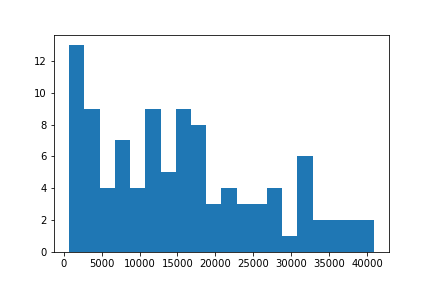
\includegraphics[width=\linewidth, height=6cm]{parabolic speed sampling.png} \caption{Parabolic speeds of study 2} \label{parabolic} \par
			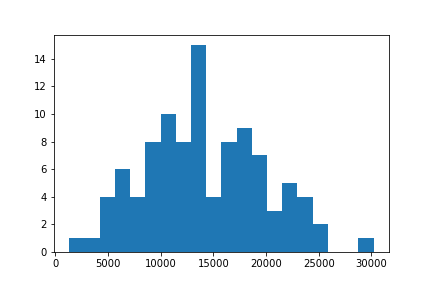
\includegraphics[width=\linewidth, height=6cm]{maxwellian speed sampling.png} \caption{Maxwellian speeds of study 3} \label{maxwellian} \par
		\end{multicols}
	\end{figure}
	\noindent On the right in figure (\ref{maxwellian}) we see the histogram of Maxwellian sampled speeds from study 2. On the left in figure (\ref{parabolic}) we see the histogram of speeds sampled from a Parabolic distribution. Both distributions have the same mean and standard deviation. One can observe that a parabolic distribution approximates the half of the Maxwellian distribution, which is why it is interesting to us. It would also be interesting to have a double parabolic distribution that would approximate the entire Maxwellian distribution.  
	\subsection{Magnetic field along a fixed axis, with constant current}
	For the first part of this study, we use the same field configurations as in the first part of study 2.\\
	\noindent \textbf{Configurations of the Electric and Magnetic Fields}
	\begin{itemize}
		\item Magnetic field due to a Helmholtz coil (number of turns: 1000 in each coil, radius: 0.1 m): for 100  steps each \\ 
		first 20A current, orientation along
		the $z$-axis [0,0,1] \\
		second -20A current, orientation along
		the $z$-axis [0,0,1] \\
		third 20A current, orientation along
		the $z$-axis [0,0,1].
		\item Electric field constantly set to 0.
	\end{itemize}
	\noindent We plot the positions and the components of positions for a particle in the plasma.
	\begin{figure}[H]
		\begin{multicols}{2}
			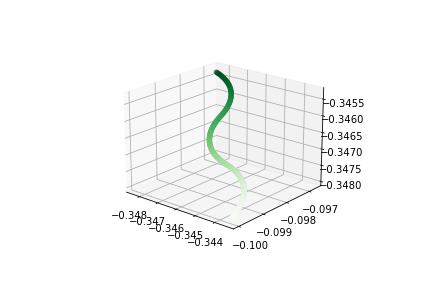
\includegraphics[width=\linewidth, height=6cm]{ps3Bz.png} \caption{position} \label{ps3Bz} \par
			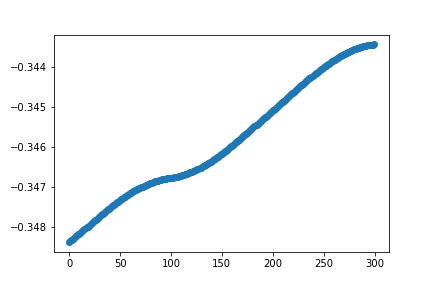
\includegraphics[width=\linewidth, height=6cm]{psx3Bz.png} \caption{$x$-component of position} \label{psx3Bz} \par
		\end{multicols}
	\end{figure}
	\begin{figure}[H]
		\begin{multicols}{2}
			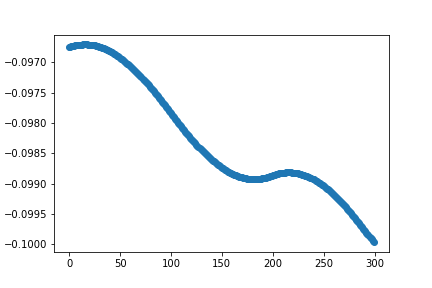
\includegraphics[width=\linewidth, height=6cm]{psy3Bz.png} \caption{$y$-component of position} \label{psy3Bz} \par
			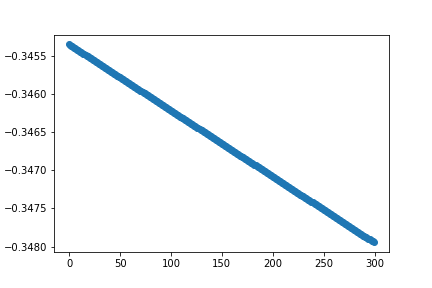
\includegraphics[width=\linewidth, height=6cm]{psz3Bz.png} \caption{$z$-component of position} \label{psz3Bz} \par
		\end{multicols}
	\end{figure}
	\noindent We also plot the velocities and the components of velocities of the same particle.
	\begin{figure}[H]
		\begin{multicols}{2}
			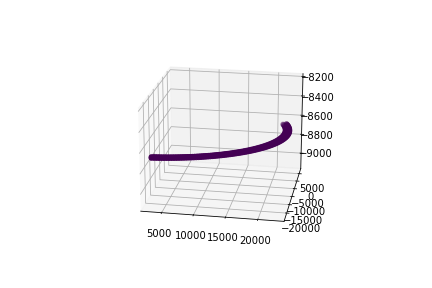
\includegraphics[width=\linewidth, height=6cm]{vs3Bz.png} \caption{velocity} \label{vs3Bz} \par
			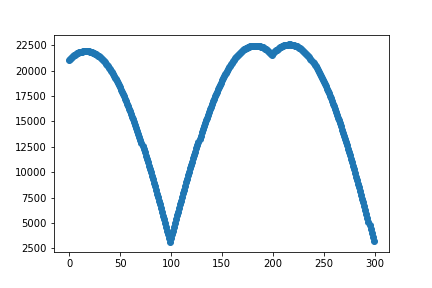
\includegraphics[width=\linewidth, height=6cm]{vsx3Bz.png} \caption{$x$-component of velocity} \label{vsx3Bz} \par
		\end{multicols}
	\end{figure}
	\begin{figure}[H]
		\begin{multicols}{2}
			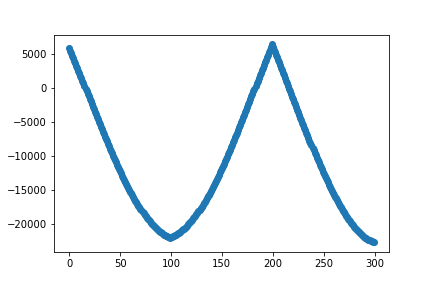
\includegraphics[width=\linewidth, height=6cm]{vsy3Bz.png} \caption{$y$-component of velocity} \label{vsy3Bz} \par
			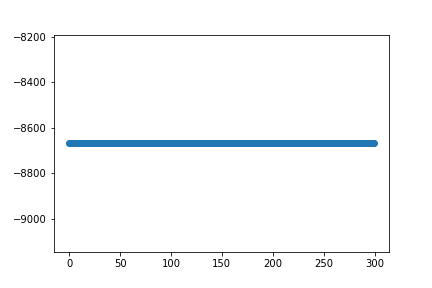
\includegraphics[width=\linewidth, height=6cm]{vsz3Bz.png} \caption{$z$-component of velocity} \label{vsz3Bz} \par
		\end{multicols}
	\end{figure}
	\noindent We see a similar behavior to the first part of study 2, because the setup of the fields are the same in this case. We also plot the positions and the components of positions for 10 particles in the plasma. Due to a bug in the program that we were unable to debug, we could not make plots for the 10 particles in the same figure, so we made them instead in different subplots. It is not the same as plotting them in the same figure, but we can also get a pretty good idea from plotting them in different subplots.
	\begin{figure}[H]
		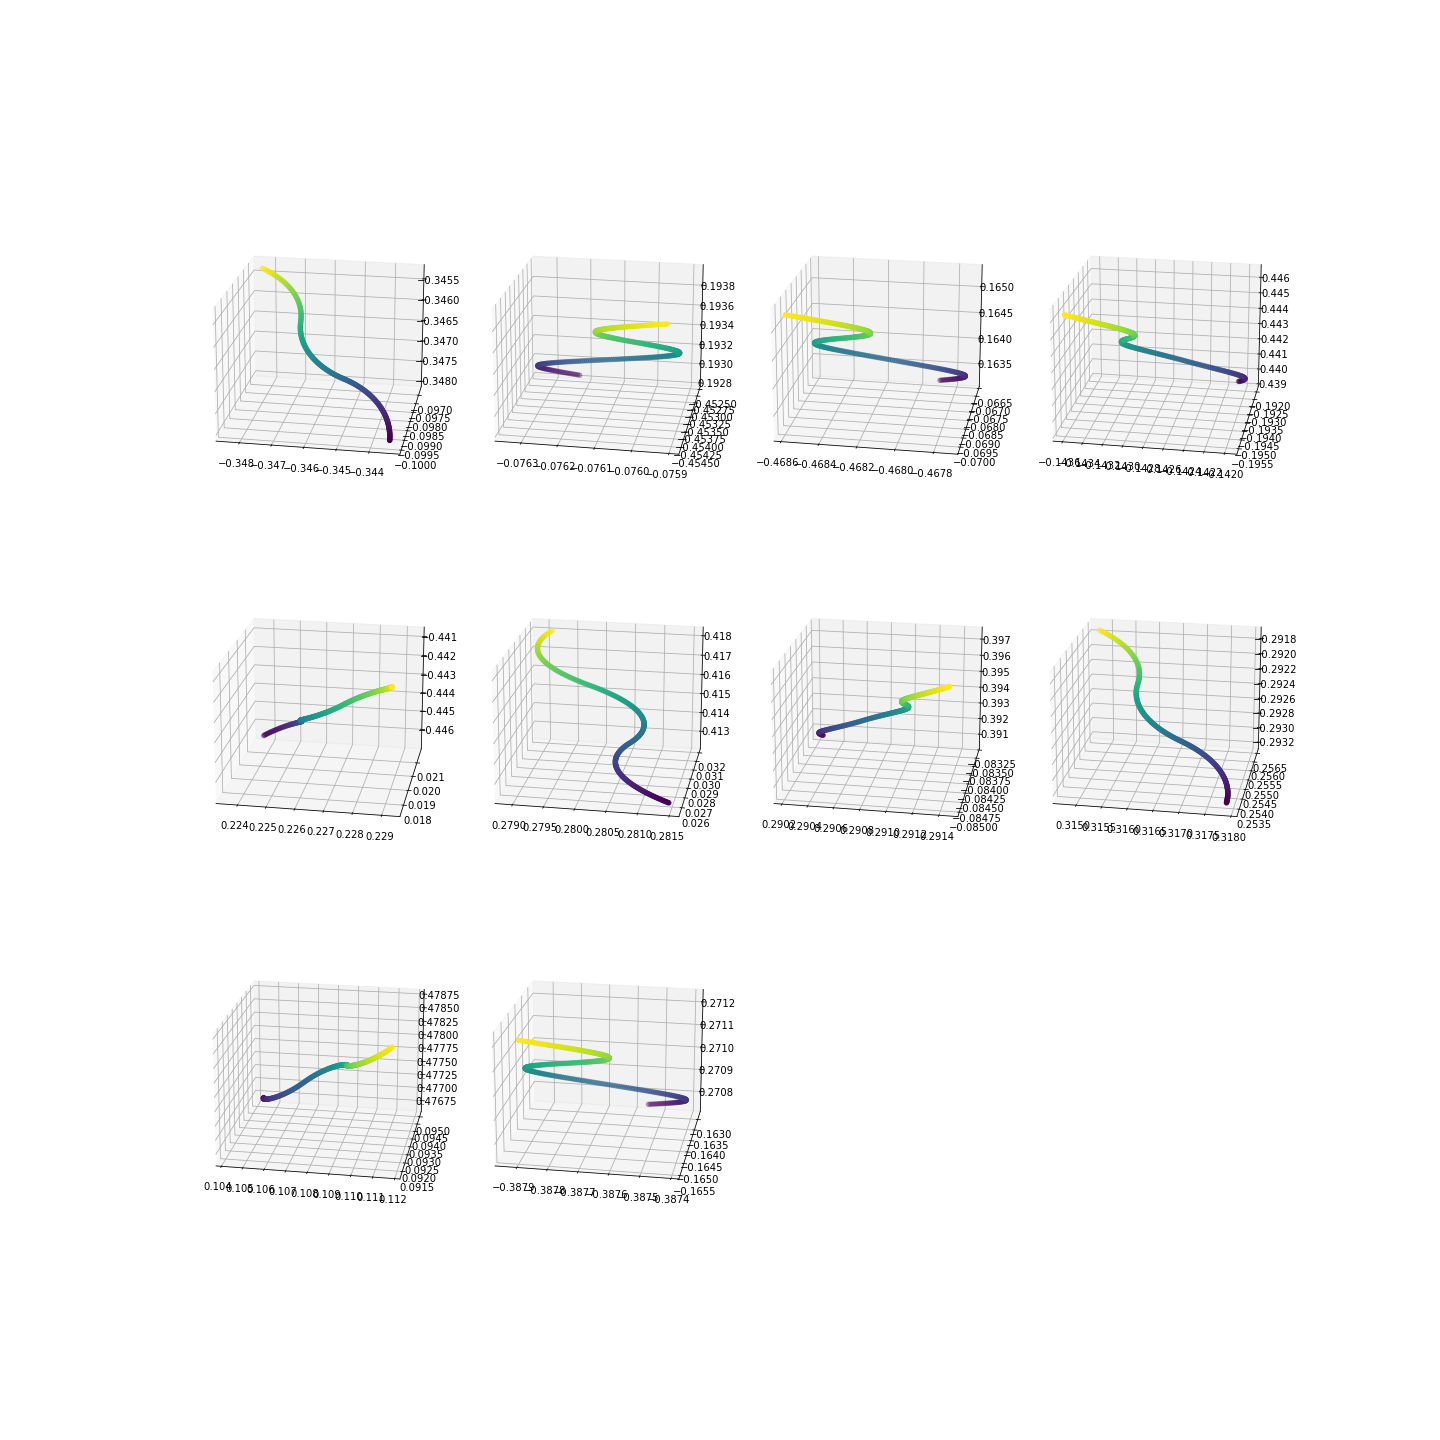
\includegraphics[width=\linewidth, height=22cm]{subps3Bz.png} \caption{positions} \label{subps3Bz}
	\end{figure}
	\begin{figure}[H]
		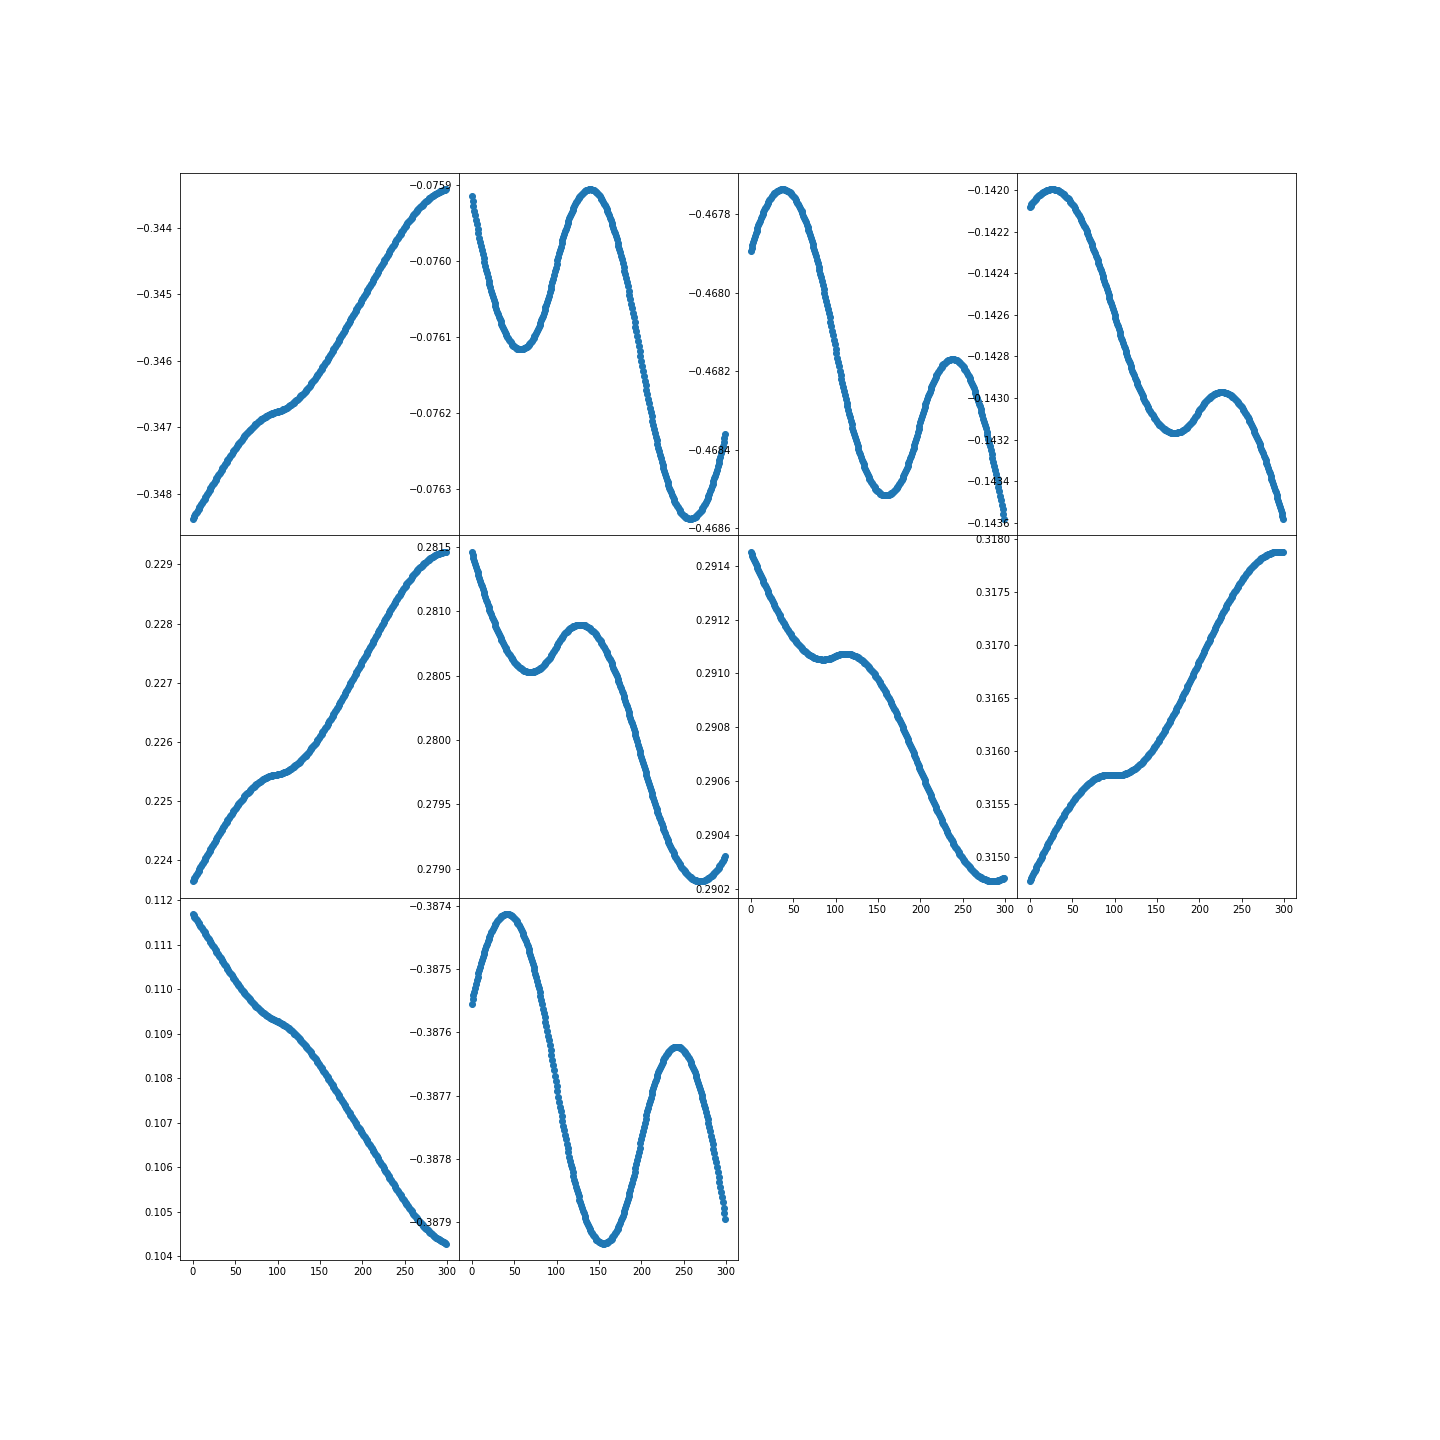
\includegraphics[width=\linewidth, height=20cm]{subpsx3Bz.png} \caption{$x$-components of positions} \label{subpsx3Bz}
	\end{figure}
	\begin{figure}[H]
		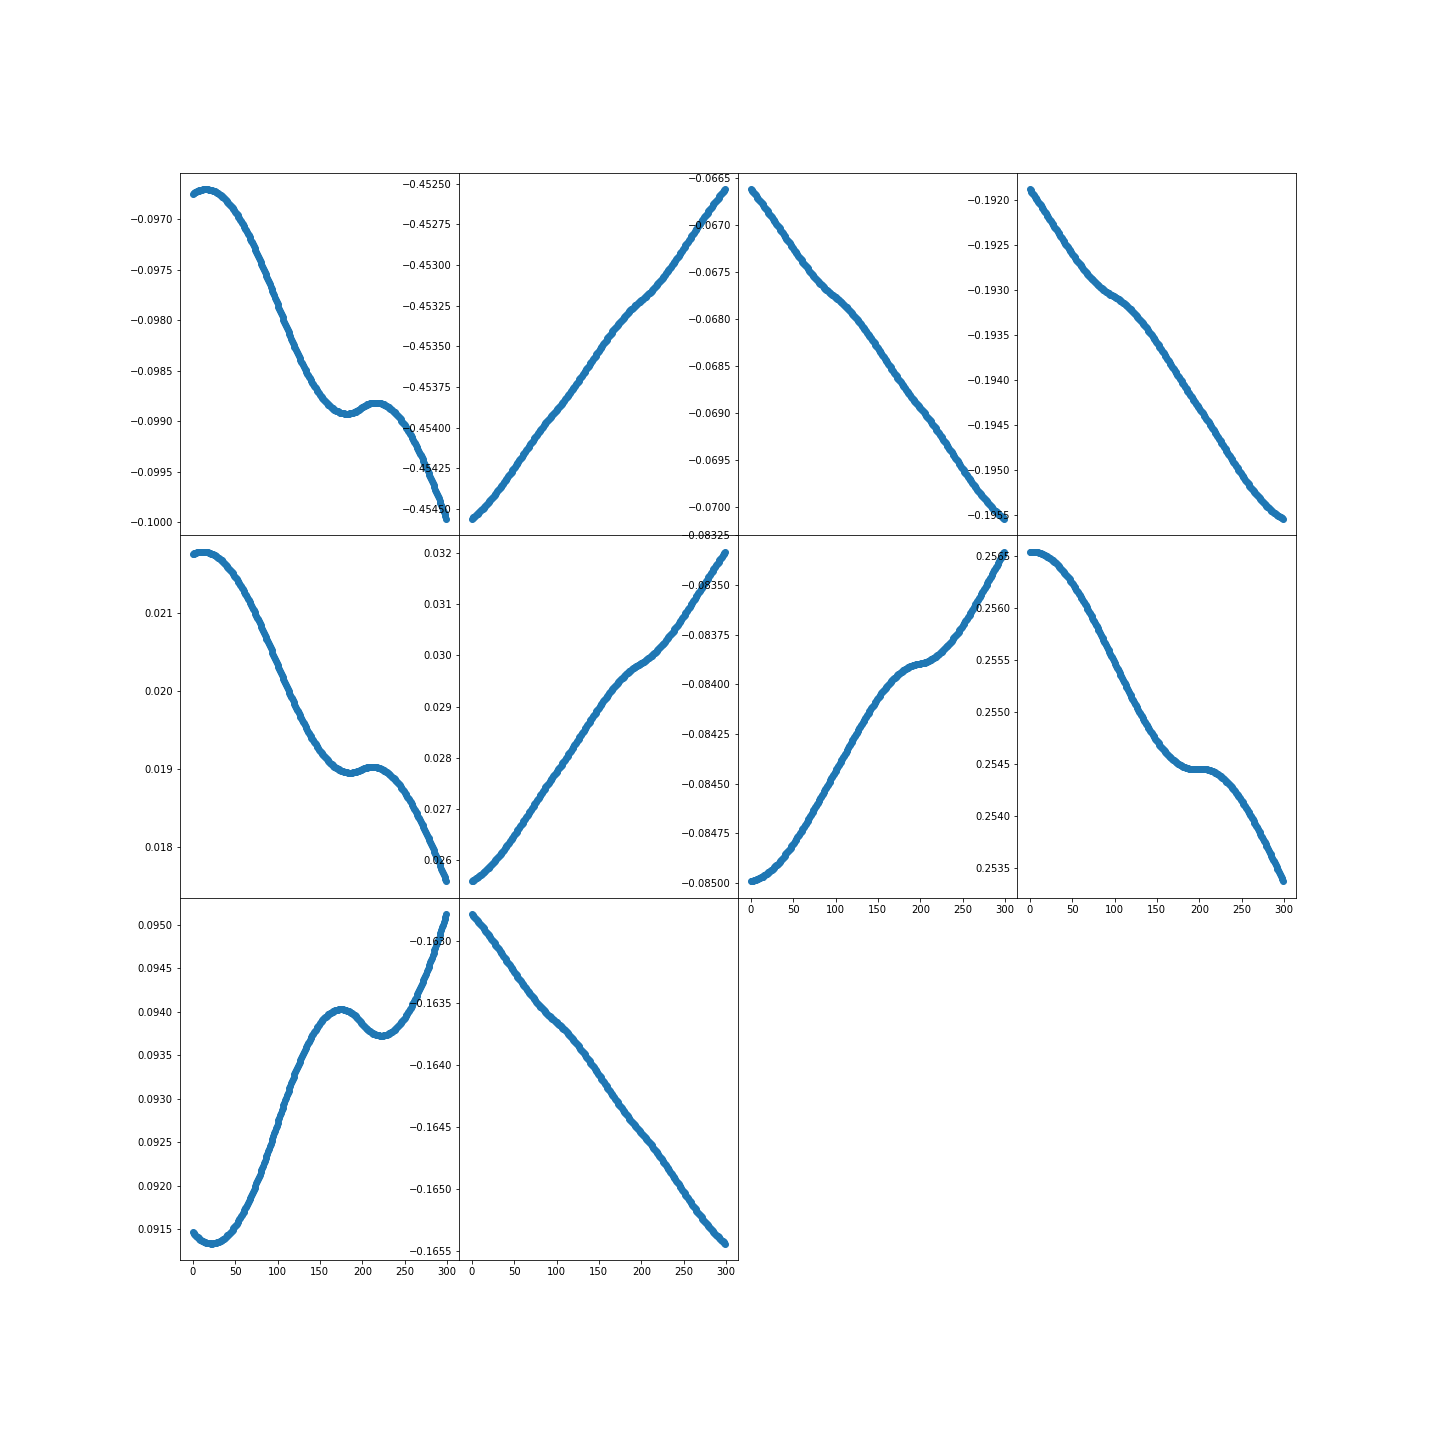
\includegraphics[width=\linewidth, height=20cm]{subpsy3Bz.png} \caption{$y$-components of positions} \label{subpsy3Bz}
	\end{figure}
	\begin{figure}[H]
		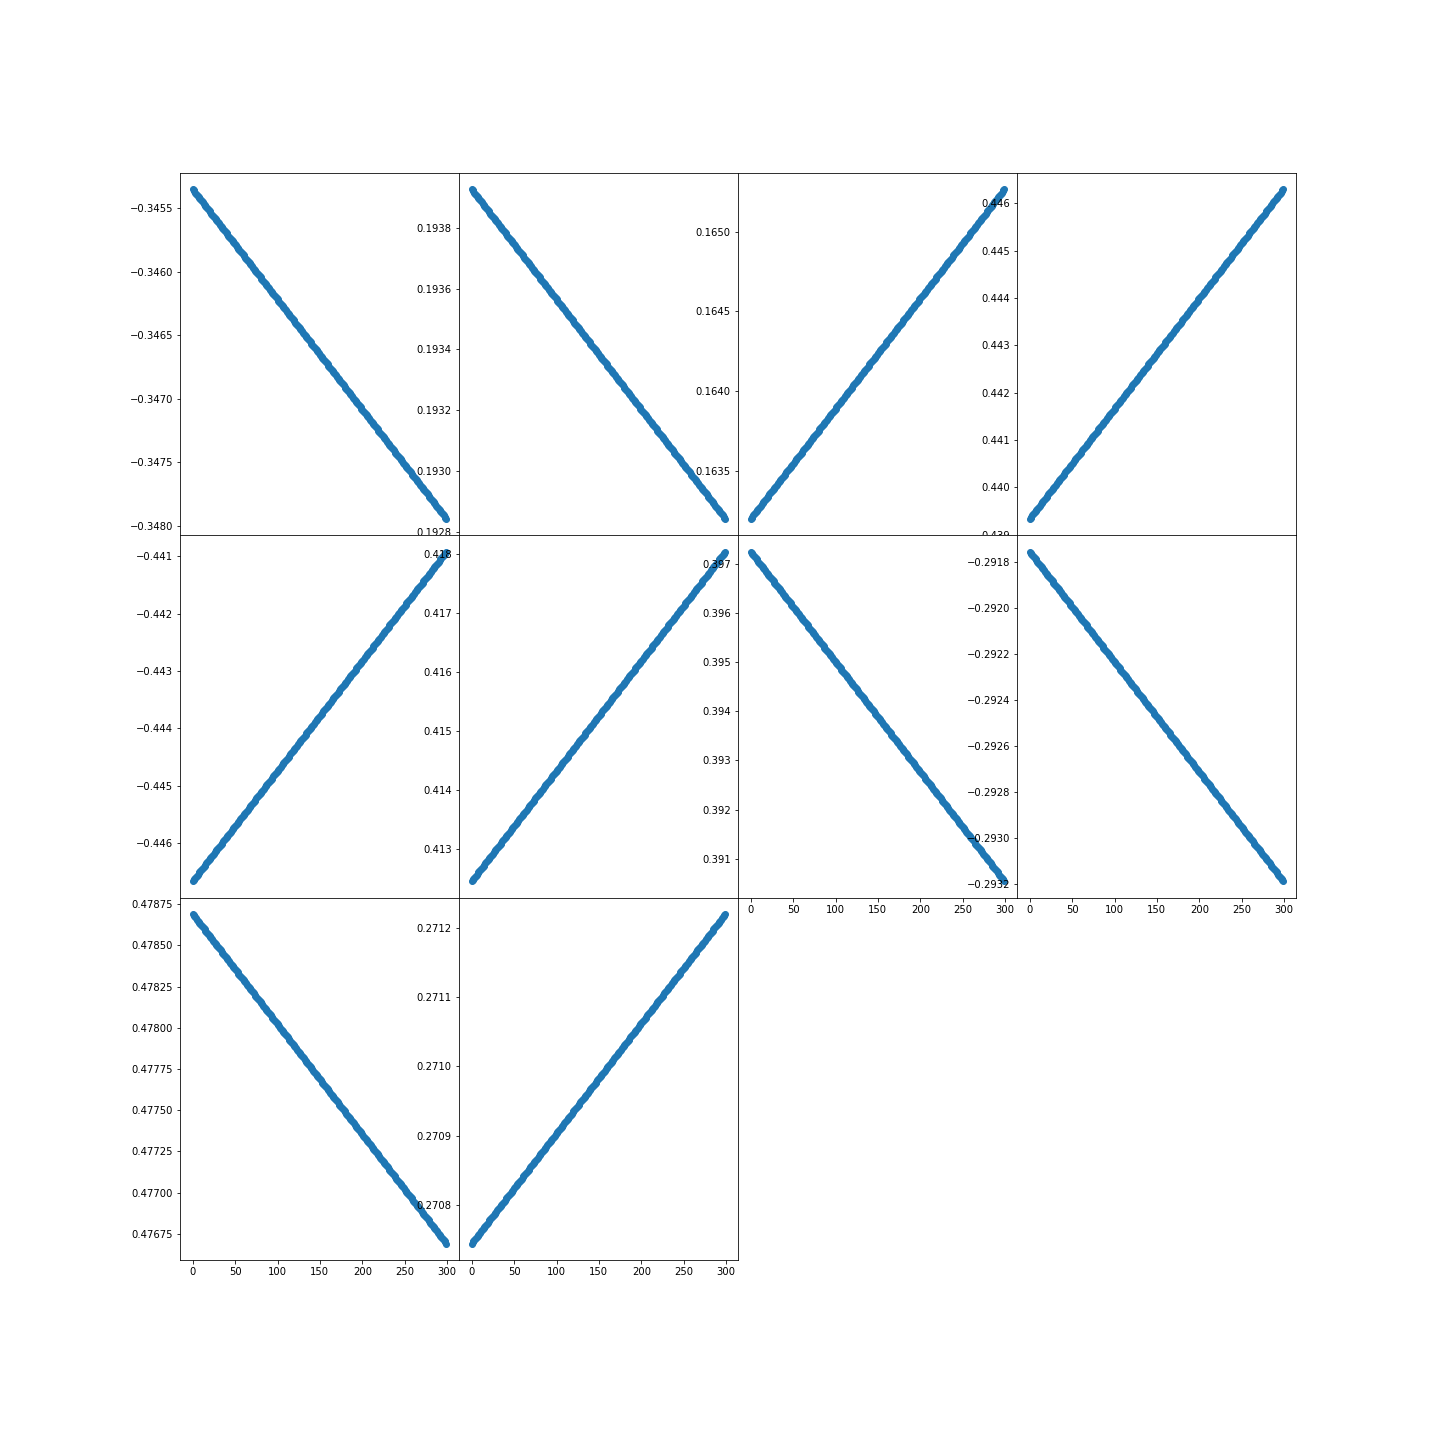
\includegraphics[width=\linewidth, height=20cm]{subpsz3Bz.png} \caption{$z$-components of positions} \label{subpsz3Bz}
	\end{figure}
	\noindent We then plot the velocities and the components of velocities for the same 10 particles.
	\begin{figure}[H]
		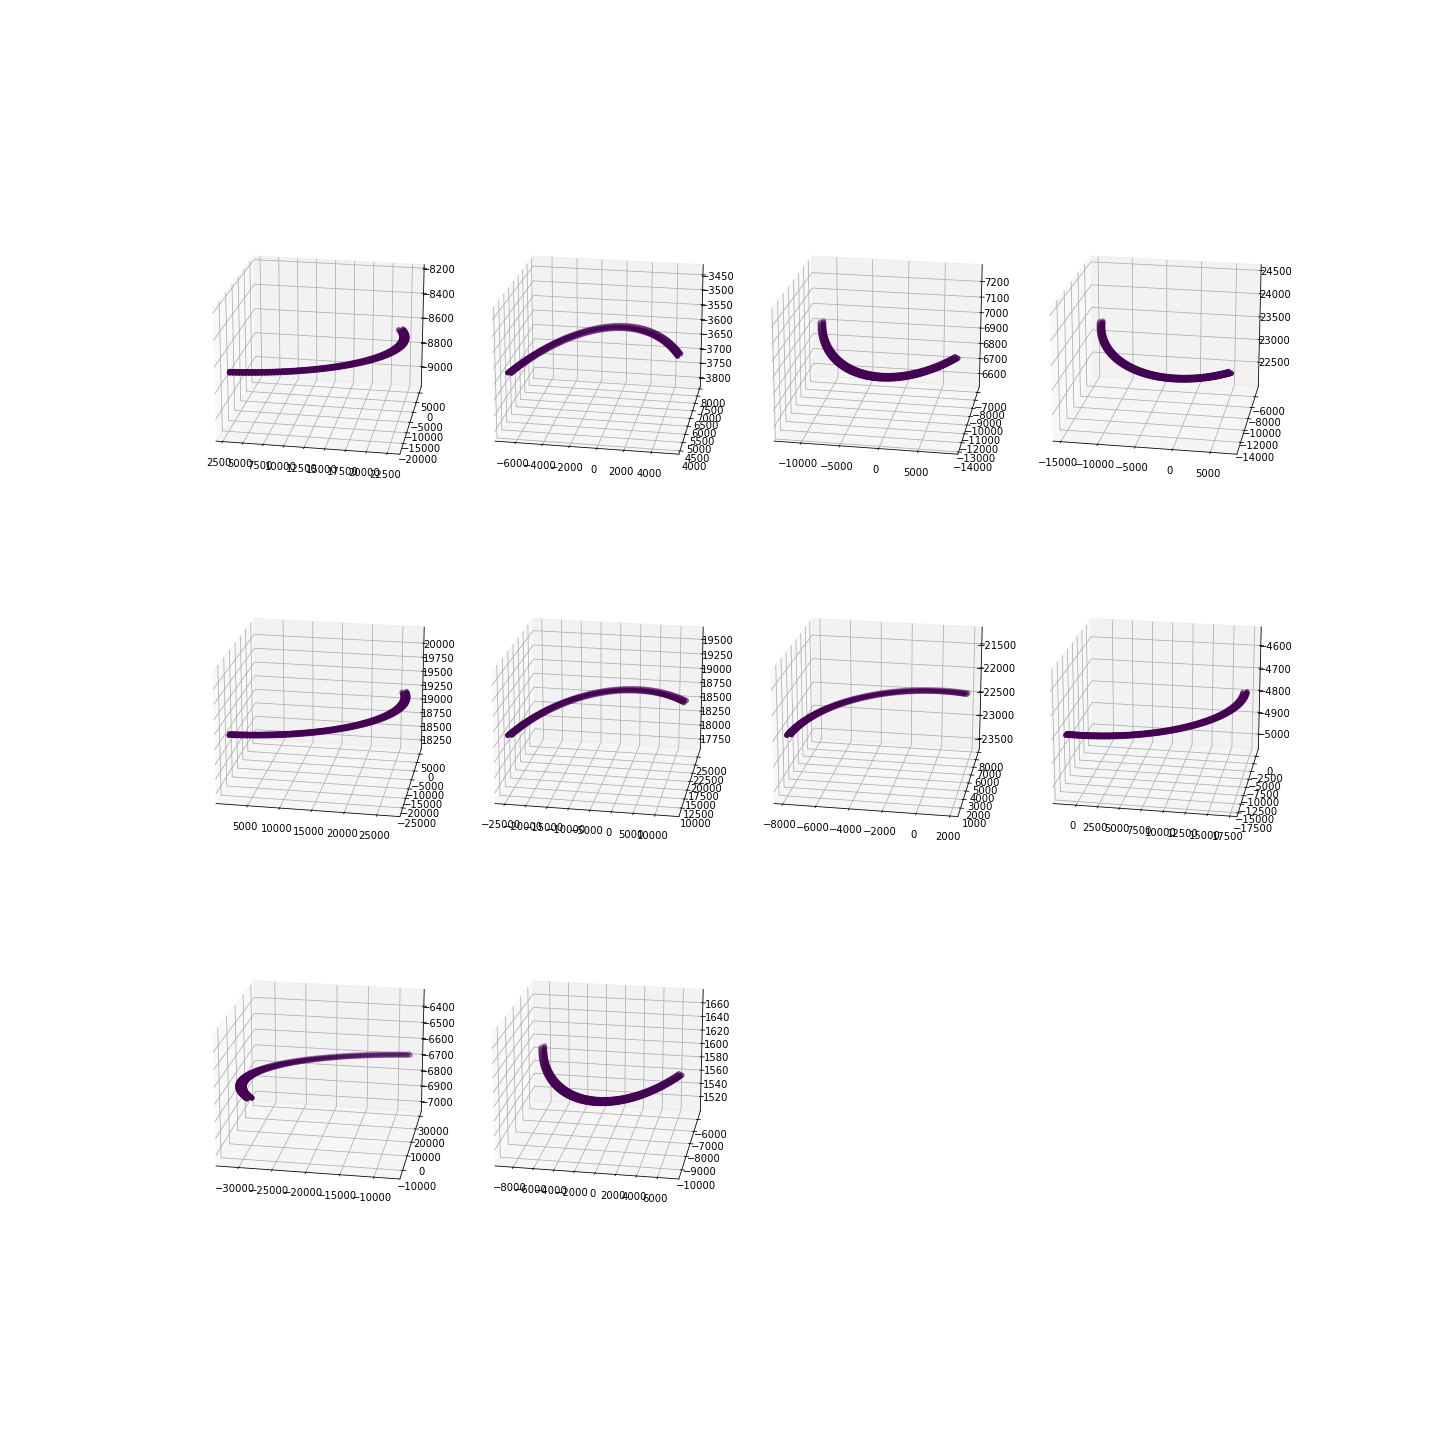
\includegraphics[width=\linewidth, height=22cm]{subvs3Bz.png} \caption{velocities} \label{subvs3Bz}
	\end{figure}
	\begin{figure}[H]
		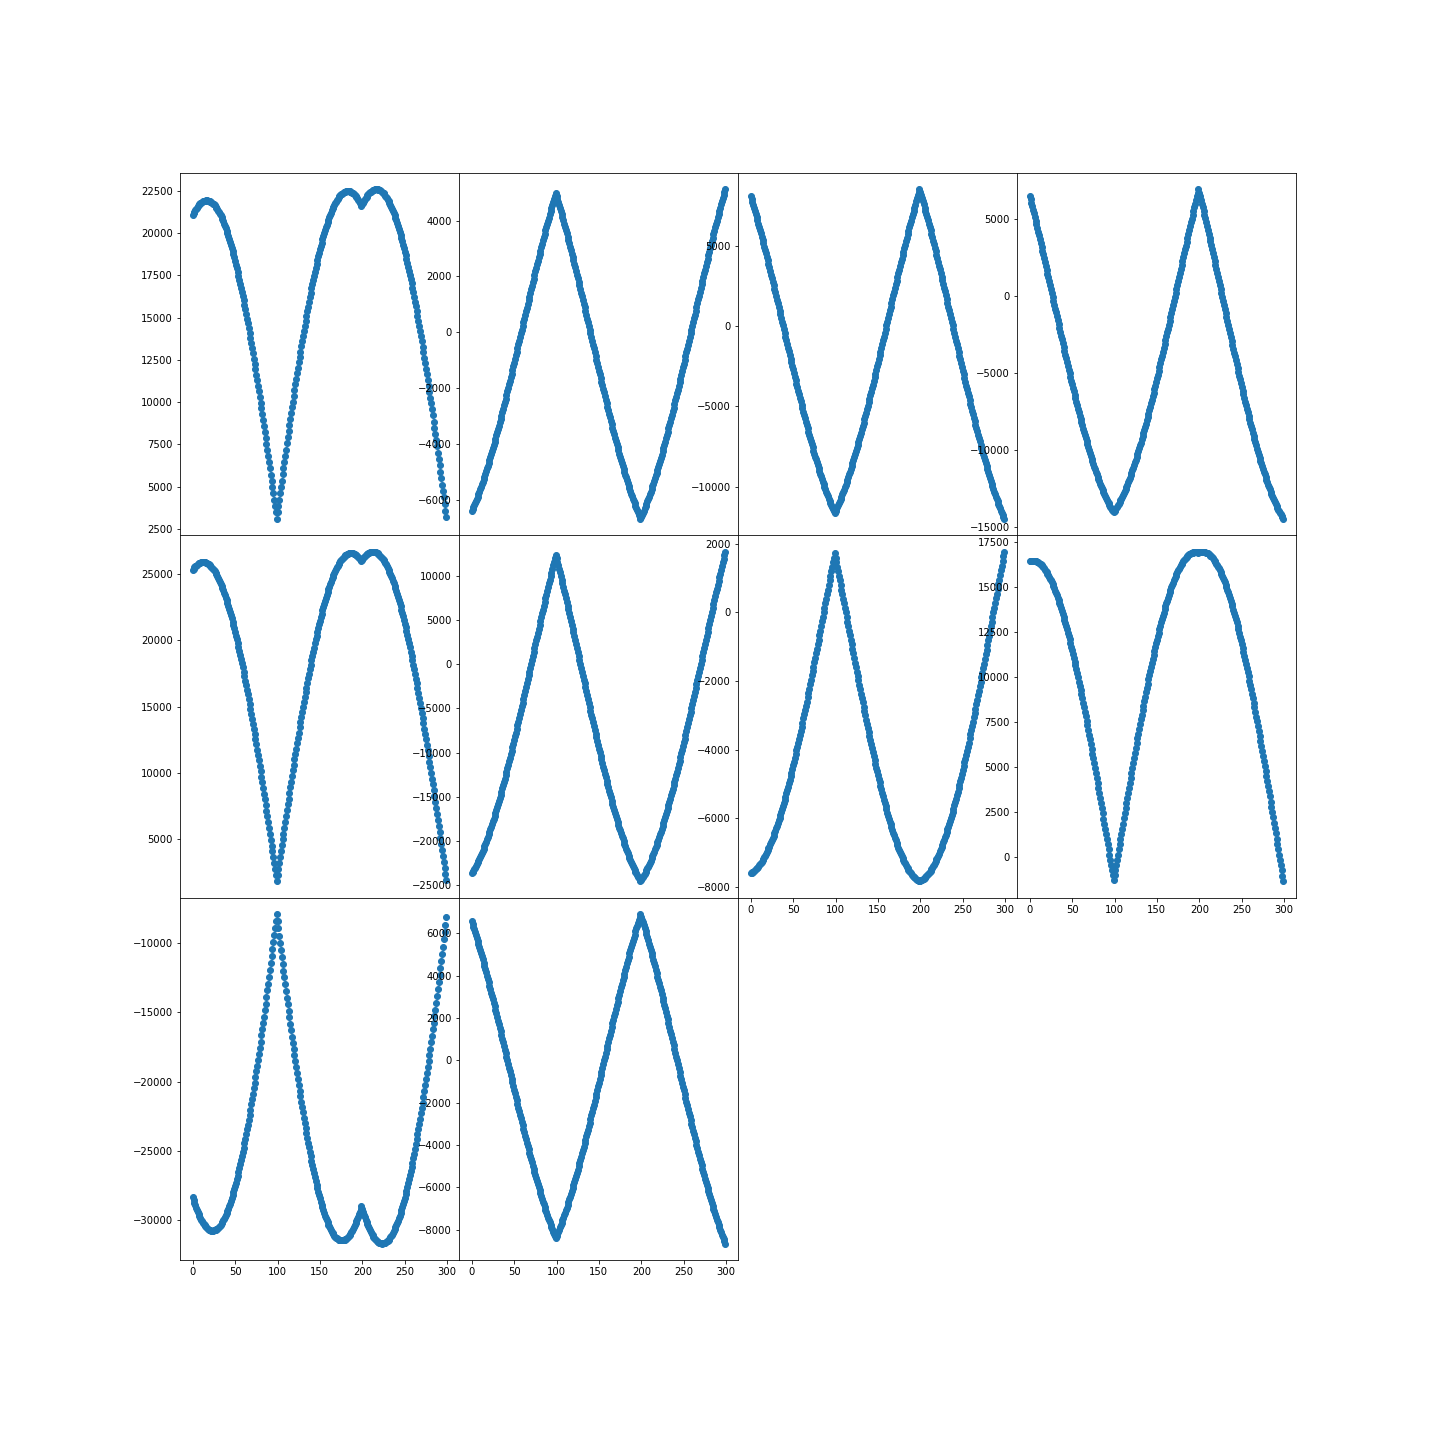
\includegraphics[width=\linewidth, height=20cm]{subvsx3Bz.png} \caption{$x$-components of velocities} \label{subvsx3Bz}
	\end{figure}
	\begin{figure}[H]
		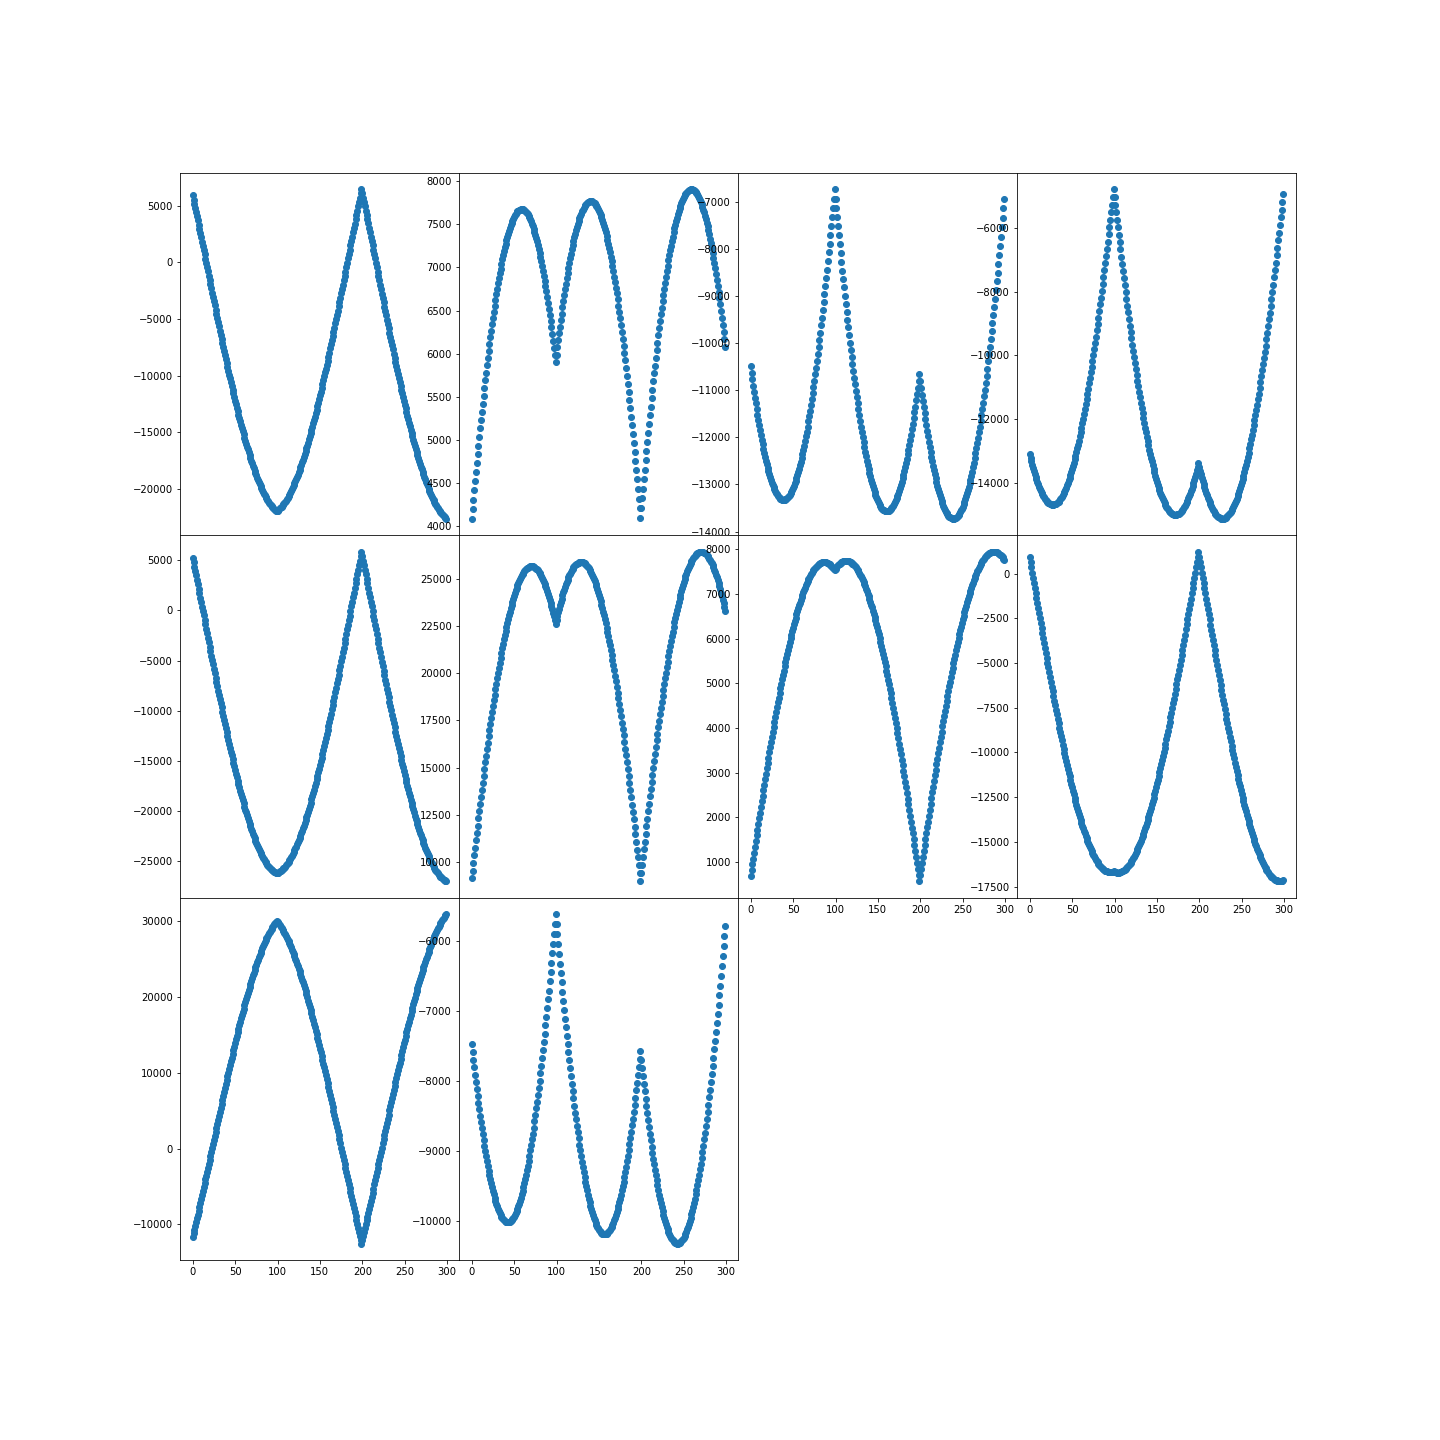
\includegraphics[width=\linewidth, height=20cm]{subvsy3Bz.png} \caption{$y$-components of velocities} \label{subvsy3Bz}
	\end{figure}
	\begin{figure}[H]
		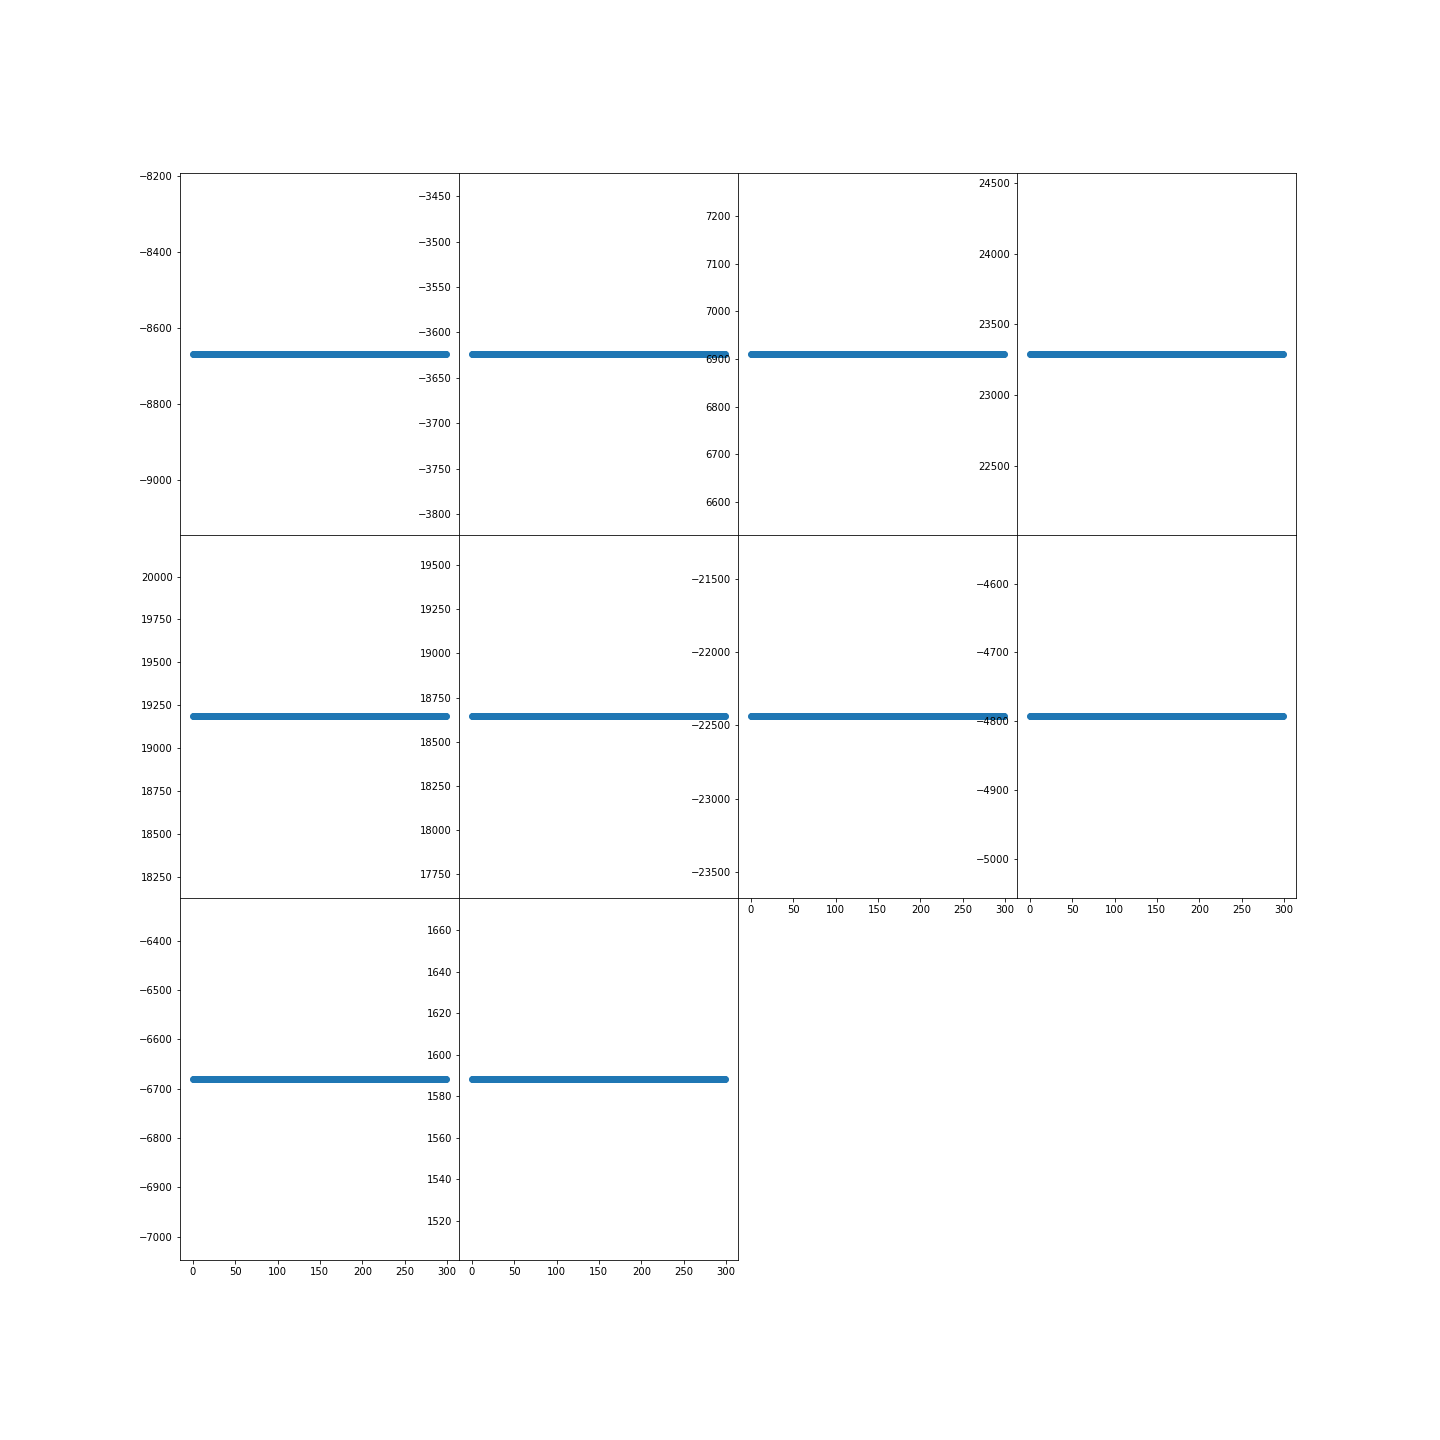
\includegraphics[width=\linewidth, height=20cm]{subvsz3Bz.png} \caption{$z$-components of velocities} \label{subvsz3Bz}
	\end{figure}
	As with the single particle, we see a similar behavior to the first part of study 2, because the setup of the fields are the same in this case. However, the particles don't all start in the same position. It is a bit more difficult to understand that the initial distribution of positions and velocities is different in this case, especially being unable to plot all the particles in the same figure.
	\subsection{Magnetic field with changing current and orientation}
	For the second part of the study, we use the same field configurations as in the second part of study 2. \\
	\noindent \textbf{Configurations of the Electric and Magnetic Fields}
	\begin{itemize}
		\item Magnetic field due to a Helmholtz coil (number of turns: 1000 in each coil, radius: 0.1 m): for 100  steps each \\ 
		first 100A current, orientation along
		the $z$-axis [0,0,1] \\
		second -20A current, orientation along the $x$-axis [1,0,0] \\
		third 50A current,
		orientation along the $y$-axis [0,1,0].
		\item Electric field constantly set to 0.
	\end{itemize}
	\noindent We first plot the positions and the components of positions for a particle in the simulation.
	\begin{figure}[H]
		\begin{multicols}{2}
			\includegraphics[width=\linewidth, height=6cm]{ps3.png} \caption{position} \label{ps3} \par
			\includegraphics[width=\linewidth, height=6cm]{psx3.png} \caption{$x$-component of position} \label{psx3} \par
		\end{multicols}
	\end{figure}
	\begin{figure}[H]
		\begin{multicols}{2}
			\includegraphics[width=\linewidth, height=6cm]{psy3.png} \caption{$y$-component of position} \label{psy3} \par
			\includegraphics[width=\linewidth, height=6cm]{psz3.png} \caption{$z$-component of position} \label{psz3} \par
		\end{multicols}
	\end{figure}
	\noindent We then plot the velocities and the components of velocities for the same particle.
	\begin{figure}[H]
		\begin{multicols}{2}
			\includegraphics[width=\linewidth, height=6cm]{vs3.png} \caption{velocity} \label{vs3} \par
			\includegraphics[width=\linewidth, height=6cm]{vsx3.png} \caption{$x$-component of velocity} \label{vsx3} \par
		\end{multicols}
	\end{figure}
	\begin{figure}[H]
		\begin{multicols}{2}
			\includegraphics[width=\linewidth, height=6cm]{vsy3.png} \caption{$y$-component of velocity} \label{vsy3} \par
			\includegraphics[width=\linewidth, height=6cm]{vsz3.png} \caption{$z$-component of velocity} \label{vsz3} \par
		\end{multicols}
	\end{figure}
	\noindent Like with the first part of study3, we see that the evolution of the particle resembles that in study 2 (the second part in this case) since the field setup is the same. We also plot the positions and the components of positions for 10 particles in the simulation. Like with the first part of study 3, we were unable to make plots for 10 particles in the same figure and had to use subplots.
	\begin{figure}[H]
		\includegraphics[width=\linewidth, height=22cm]{subps3.png} \caption{positions} \label{subps3}
	\end{figure}
	\begin{figure}[H]
		\includegraphics[width=\linewidth, height=20cm]{subpsx3.png} \caption{$x$-components of positions} \label{subpsx3}
	\end{figure}
	\begin{figure}[H]
		\includegraphics[width=\linewidth, height=20cm]{subpsy3.png} \caption{$y$-components of positions} \label{subpsy3}
	\end{figure}
	\begin{figure}[H]
		\includegraphics[width=\linewidth, height=20cm]{subpsz3.png} \caption{$z$-components of positions} \label{subpsz3}
	\end{figure}
	We the plot the velocities and the components of velocities for the same 10 particles.
	\begin{figure}[H]
		\includegraphics[width=\linewidth, height=22cm]{subvs3.png} \caption{velocities} \label{subvs3}
	\end{figure}
	\begin{figure}[H]
		\includegraphics[width=\linewidth, height=20cm]{subvsx3.png} \caption{$x$-components of velocities} \label{subvsx3}
	\end{figure}
	\begin{figure}[H]
		\includegraphics[width=\linewidth, height=20cm]{subvsy3.png} \caption{$y$-components of velocities} \label{subvsy3}
	\end{figure}
	\begin{figure}[H]
		\includegraphics[width=\linewidth, height=20cm]{subvsz3.png} \caption{$z$-components of velocities} \label{subvsz3}
	\end{figure}
	\noindent Like we discussed in the first part of study 3, it is difficult to tell that the initial distribution of positions and velocities are very different from those in study 2, especially having different particles in different figures. However, one can notice in figures (\ref{subps3}) and (\ref{subvs3}) that the evolution paths look more diverse among themselves than those in study 2; which is suggestive that initial particle position and velocity distribution is different in study 3 than in study 2.
	\section{Prospects for such studies}
	\noindent We have also made animations for the plots which help us understand the evolution of the particles in the plasma even better. Due to the limitation of time, we were only able to perform these studies. Should one spend a few more months on such a project, many interesting studies could be done, including studies that really help one use plasma devices better during plasma processes such as those in surface engineering practices. 
	
	\noindent Some interesting studies that could be done, by building on the available resources could be:
	\begin{itemize}
		\item Define new field configurations; either analytical or based on expressions that mimic coils or instruments used to create fields.
		\item Vary the fields (either slowly or abruptly)and see how the particles evolve.
		\item Define new distributions to sample the initial position and velocity distributions.
		\item Use different distributions in the same study to mimic particles entering the chamber through multiple routes.
		\item Save the states of the particles at some point in the study and use that as initial distribution for another study.
		\item Allow functionality to absorb particles (in coating processes) or eject particles from the chamber.
		\item Define interactions between the particles.
		\item Create an interactive plasma simulation which keeps running on a computer and the user input can change the particles, fields and other properties of the simulation.
		\item Study the effect of plasma temperature on certain plasma processes.
		
	\end{itemize}
		
	\noindent Study 1 mostly served the purpose of showing that the program works well. In study 1, we kept the magnetic field to be constant, while we changed the electric field. In study 2 we set out to study how we can control particles in a plasma by controlling the magnetic field, as that closely follows the aim of our project. We first see that we can completely trap the particles along the magnetic field. In the second part of study 2, we see that by changing the direction of the magnetic field, we can trap the particles in any direction we want to. In summary, possibly using a coil whose orientation we can change, we can create a magnetic trap for a plasma chamber. By controlling the current in the coil and its orientation, we can control plasma very well. And we can also do studies based on such a setup. Although we did not the study specifically the magnetic mirror effect, we were able to study magnetic traps for plasma. In study 3, we used a different initial distribution of the velocities and positions for particles when they enter the chamber. Initial distribution of positions describes where the particles are injected into the chamber. For example, maybe they are all injected at the same position through a port or valve like in study 2, or maybe they are sprayed through the walls or maybe we study the flux of particles reflected off of the wall of the chamber like in study 3. The velocity distribution of the particles entering the chamber also help us understand parameters like plasma temperature. We have changed fields in a few epochs in these studies so that we can clearly notice these changes in the plots. Other strategies like changing the fields smoothly or slowly, would be difficult to observe well in the plots; although they would be very interesting from computational perspective. We did not do any computational study in our project, due to the limitation of time. We were only able to understand basic ideas about controlling plasma with electric and magnetic fields through plots. But with some extensions to a project like ours, one could perform computational studies and understand optimization techniques to model and operate the behavior or a real plasma device; which would be very useful in understanding plasma processes in surface engineering techniques. This was our motivation for the project. But we were only able to accomplish this in the time we had. However, we feel very excited about the possibilities offered by such a project. One might even find it interesting to work on such a project, during the course of one's Phd or professional academic research; and many people around the world have done so.

\begin{thebibliography}{}
	\bibitem{blog} Florian LB (GitHub user). \textit{Charged Particle Trajectories in Electric and Magnetic Fields}. Thu, 28 Jan 2016. \textit{https://flothesof.github.io/charged-particle-trajectories-E-and-B-fields.html}
	\bibitem{scipyRdist} Scipy library rdist distribution documentation. \textit{https://docs.scipy.org/doc/scipy/reference/generated/scipy.stats.rdist.html}
\end{thebibliography}
\end{document}